\begin{frame}\begin{center}
\LARGE\textbf{Matching}
\end{center}\end{frame}
%-------------------------------------------------------------------------------
%-------------------------------------------------------------------------------
\begin{frame}\textbf{Key Identifiying Assumption}

\begin{align*}
(Y_1, Y_0)\indep D\mid X \\
\end{align*}

What is in the agent's and econometrician's information set?

\begin{itemize}\setlength\itemsep{1em}
\item \citeA{Navarro.2004} highlights the sensitivity of results to different conditioning variables.
\end{itemize}
\end{frame}
%-------------------------------------------------------------------------------
%-------------------------------------------------------------------------------
\begin{frame}
\begin{figure}\caption{Matching and Essential Heterogeneity}
\scalebox{0.35}{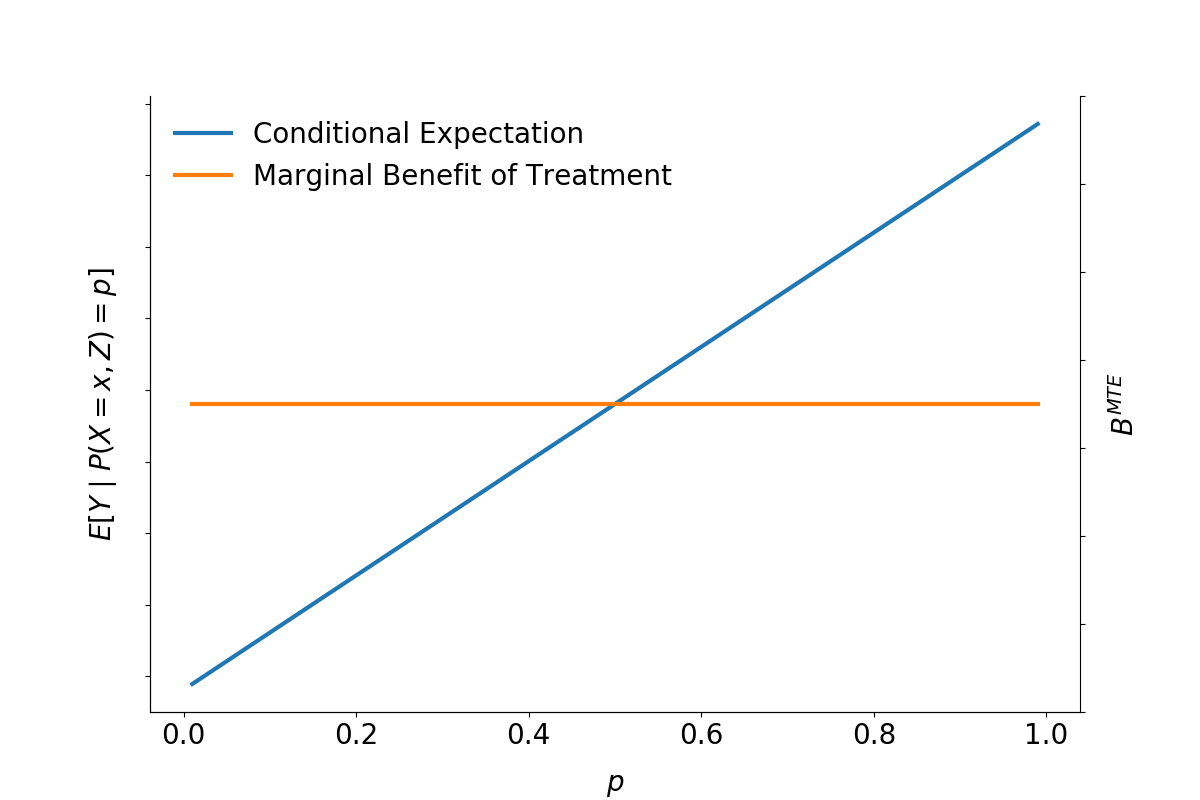
\includegraphics{fig-strategy-matching}}
\end{figure}
\end{frame}
%-------------------------------------------------------------------------------
%-------------------------------------------------------------------------------
